\section{Introduction}

\subsection{Web Service}

\begin{frame}
%\transsplithorizontalout[duration=1]
%\transboxin[duration=1]
%\transboxout[duration=1]
%\transblindshorizontal[duration=1]
%\transblindsvertical[duration=1]
%\transglitter[duration=1]
%\transsplitverticalin[duration=1]port fermet
\transsplitverticalout[duration=1.5]
%\transsplithorizontalout[duration=1]
%\transwipe[duration=1]%haut au bas
\frametitle{Introduction}
\framesubtitle{Web service}
\begin{block}{Définition}
\begin{itemize}
\item Il s'agit d'une technologie permettant à des applications de dialoguer à distance via Internet, et ceci indépendamment des plates-formes et des langages sur lesquelles elles reposent. Pour ce faire, les services Web s'appuient sur un ensemble de protocoles Internet très répandus (\textcolor{deepblue}{XML}, \textcolor{deepblue}{HTTP}), afin de communiquer.
\end{itemize}
\end{block}
\end{frame}


\begin{frame}
\transsplithorizontalout[duration=1]
\frametitle{Introduction}
\framesubtitle{Web service}
\begin{itemize}
\item[\textcolor{blue}{$\blacktriangleright$}]<1-> Les Web Services proposent aux utilisateurs du Web des fonctionnalités pratiques grâce à un protocole Web standard (dans la plupart des cas, le protocole utilisé est \textcolor{deepblue}{SOAP}).
\item[\textcolor{blue}{$\blacktriangleright$}]<2-> Les Web Services offrent un moyen de décrire leurs interfaces à l'aide d'un document \textcolor{deepblue}{XML} nommé \textcolor{deepblue}{WSDL} (Web Services Description Language) qui précise les méthodes pouvant être invoquées, leurs signatures et les points d'accès du service (URL, port ...).
\item[\textcolor{blue}{$\blacktriangleright$}]<3-> Grâce à \textcolor{deepblue}{UDDI} (Universal Discovery Description and Integration), les utilisateurs potentiels peuvent trouver facilement le web service.
\item[\textcolor{colname}{$\blacktriangleright$}]<4-> Les services Web sont accessibles via \textcolor{deepgreen}{SOAP}, la requête et les réponses sont des messages \textcolor{deepblue}{XML} transportés sur \textcolor{deepblue}{HTTP}.
\end{itemize}
\end{frame}


\subsection{Etudiant web service}
\begin{frame}
\frametitle{Introduction}
\framesubtitle{Etudiant web service}
\transsplithorizontalout[duration=1]

Ce service permet aux étudiants de se connecter  avec leurs CNE comme login et leurs noms par défaut comme mot de passe. Une fois l'étudiant est connecté peut:
\begin{itemize}
\item[\textcolor{colname}{$\bigstar$}]<1-> Visualiser ses informations personnelles.
\item[\textcolor{colname}{$\bigstar$}]<2-> Poursuivre ses modules actuels. (note, rattrapage, professeur, ...).
\item[\textcolor{colname}{$\bigstar$}]<3-> Consulter sa situation pédagogique. (Modules déjà validés).
\item[\textcolor{colname}{$\bigstar$}]<4-> Découvrir la liste des professeurs de ses modules actuels. (nom complet, téléphone, email).
\item[\textcolor{colname}{$\bigstar$}]<5-> Modifier son adresse, son email, son téléphone, et son mot de passe.
\item[\textcolor{colname}{$\bigstar$}]<6-> Avoir une idée générale sur le contenu de la formation. 
\end{itemize}

\end{frame}

\section{Outils}
\subsection{Framework Django}
\begin{frame}
\frametitle{Framework Django}
\transboxout[duration=1]
\begin{columns}
\begin{column}{6.5cm}
\begin{exampleblock}{Définition}<2->
\begin{itemize}
\item \textcolor{backgroundcolor}{\textbf{Django}} est un framework open-source de développement web en 
\textcolor{colorPython}{Python}.
\item Il a pour but de rendre le développement web \textcolor{red}{2.0} simple et 
rapide.
\item Aujourd'hui, \textcolor{backgroundcolor}{\textbf{Django}} est devenu très populaire et est utilisé 
par des sociétés du monde entier, telles qu'Instagram, Pinterest, et 
la NASA.
\end{itemize}
\end{exampleblock}
\end{column}
\begin{column}{3.5cm}

\includegraphics[width=3.5cm,height=2cm]{images/django.png}
\end{column}
\begin{column}{6.5cm}
\begin{exampleblock}{Versions}<3->
\vspace*{0.8cm}
\begin{itemize}
\item La version supporté est la version actuelle \textcolor{red}{1.9} sortie le 1er décembre 
2015 compatible avec \textcolor{colorPython}{Python} \textcolor{red}{2.7}, \textcolor{red}{3.4} et \textcolor{red}{3.5}. La version à venir est \textcolor{red}{1.10} sera sortir dans Juillet 2016.
\end{itemize}
\vspace*{2cm}
\end{exampleblock}
\end{column}
\end{columns}
\begin{columns}
\begin{column}{15cm}
\begin{block}{}<4->
\begin{itemize}
\item Liens de documentation: \textcolor{urlcolor}{\url{https://docs.djangoproject.com/fr/1.9}}\\
\item  Télécharger depuis: \textcolor{urlcolor}{\url{https://www.djangoproject.com/download/}}
\end{itemize}
\end{block}
\end{column}
\end{columns}
\end{frame}

\begin{frame}
\frametitle{Framework Django}
\framesubtitle{MVT}
\transwipe[duration=1]
\begin{itemize}
\item[\textcolor{blue}{$\blacktriangleright$}] Le framework \textcolor{backgroundcolor}{\textbf{Django}} utilise l'architecture \textcolor{backgroundcolor}{\textbf{MVT}}: Modèle-Vue-Template.
\end{itemize}
\begin{columns}
\begin{column}{11cm}
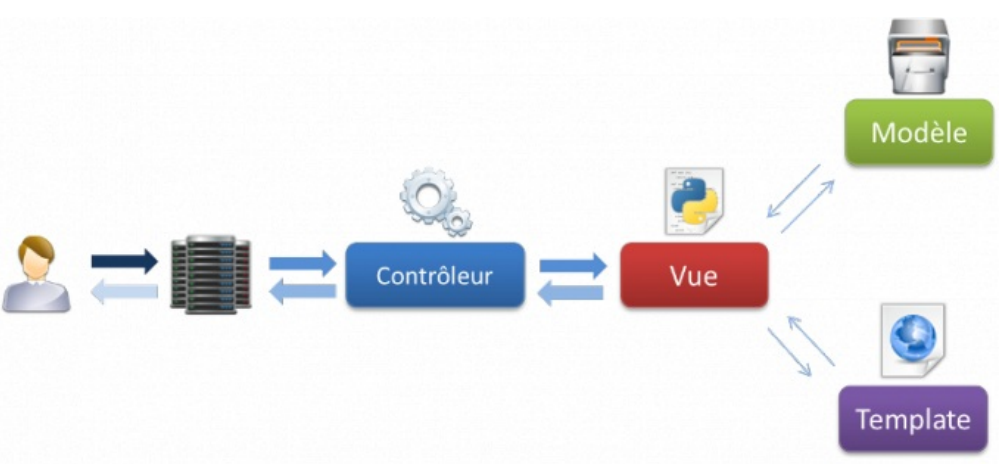
\includegraphics[width=11cm,height=5cm]{images/mvt.png}
\end{column}
\end{columns}
\end{frame}

\subsection{Soaplib}
\begin{frame}
\frametitle{Soaplib}
\framesubtitle{Définition}
\transwipe[duration=2]
\begin{columns}
\begin{column}{8.5cm}
\begin{block}{Définition}<1->
\vspace*{0.1cm}
\begin{itemize}
\item[•] \textcolor{deepgreen}{Soaplib} est une bibliothèque Python facile à utiliser pour la publication des services Web \textcolor{deepred}{SOAP} utilisant \textcolor{deepred}{WSDL 1.1} standard, et la réponse aux demandes \textcolor{deepred}{SOAP 1.1}. 
\item[•] Avec un peu de code, \textcolor{deepgreen}{Soaplib} permet d'écrire un service Web utile et le déployer comme une application \textcolor{deepblue}{WSGI}.
\vspace*{0.3cm}
\end{itemize}
\end{block}
\end{column}
\begin{column}{8.5cm}
\begin{block}{soaplib 2.0.0-beta2}<2->
\vspace*{0.2cm}
\begin{itemize}
\item[•] Publié le 2011-03-15.
\item[•] Disponible à télécharger dans :\\
\textcolor{urlcolor}{\url{https://pypi.python.org/pypi/soaplib/2.0.0-beta2}}\\
\item[•] Documentation officielle:\\
\textcolor{urlcolor}{\url{http://soaplib.github.io/soaplib/2_0/}}
\end{itemize}
\vspace*{0.3cm}
\end{block}
\end{column}
\end{columns}
\end{frame}

\subsection{Java Client Web Service}
\begin{frame}
\frametitle{Java Client Web Service}
\framesubtitle{JAX-WS }
\transwipe[duration=2]
\begin{columns}
\begin{column}{8cm}
\begin{block}{Définition}<1->
\begin{itemize}
\item[•] \textcolor{deepblue}{JAX-WS} (\textcolor{colname}{Java} API for \textcolor{colname}{XML} Web Services) est une API \textcolor{colname}{Java} pour la création des web services.
\item[•] \textcolor{deepblue}{JAX-WS} est l'une des APIs de la programmation \textcolor{colname}{Java/XML}.
\item[•] Elle fait partie du platform \textcolor{colname}{JEE} de SUN Microsystems.
\end{itemize}
\end{block}
\end{column}
\begin{column}{8cm}
\begin{block}{JAX-WS 2.2.10}<2->
\vspace*{0.1cm}
\begin{itemize}
\item[•] Publié le 2015-01-14.\\
\item[•] Disponible à télécharger dans :\\
\textcolor{urlcolor}{\url{https://jax-ws.java.net/2.2.10/}}\\
\item[•] Documentation officielle:\\
\textcolor{urlcolor}{\url{https://jax-ws.java.net/nonav/2.2.10/docs/index.html}}
\end{itemize}
\vspace*{0.2cm}
\end{block}
\end{column}
\end{columns}

\end{frame}